\section{Finite Difference Time Domain}
\label{sec:fdtd}

\begin{aautop}
    This section will describe the finite difference time domain method. This is a method for solving Maxwell equations in time domain. A brief introduction to Maxwell's Equations is given in order to understand the methodology of FDTD. After this, the techniques and ideas behind FDTD are presented and used on the 1D scalar wave-equation. An introduction to the Yee Algorithm, Yee cells, and Yee notation is presented and applied on the 3D Maxwell curl equation. Lastly, the key parameters of FDTD are discussed and related to CST Microwave Studio.
\end{aautop}

\subsection{Introduction to Maxwell's Equations}
Maxwell's equations are a set of equations that describe how electric and magnetic fields propagate. The set of equations consists of Gauss' law, Gauss' Magnetism law, Faraday's law, and finally Ampere's law. 

\subsubsection{Gauss' Law}
Gauss' law describes how the electric field behaves around electric charges. Below is Gauss' law written in point-differential form. The equation states that the divergence of the electric flux density $\bold{D}$ is equal to the volume electric charge density $\rho_V$ \cite{taflove2000computional}. This states that the field around a point $\bold{D}$ is equal to the electric charge density $\rho_V$. From this, it is found that, if there exists an electric charge, the divergence of $\bold{D}$ is nonzero, and only zero when there is no charge present. 
\begin{align}%%
\nabla \cdot \bold{D} &= \rho_V
\end{align}

\subsubsection{Gauss' Magnetism Law}
Gauss' magnetism law, is much like the previous formula, but for magnetic fields. Basically, Gauss' law for magnetism states that a magnetic charge does not exist. This is given in the Equation below \cite{taflove2000computional}. 
\begin{align}%%
\nabla \cdot \bold{B} &=0
\end{align}
From this, it is clear, that there are no magnetic monopoles. The divergence of $\bold{B}$ or $\bold{H}$ fields is always zero and the magnetic fields always flows in closed loops. 

\subsubsection{Faraday's Law}%%
Faraday's law states that the curl of the $\bold{E}$, is equal to the rate of change of a magnetic field. This is very important in the way that electric waves propagate. This is given in the Equation below \cite{taflove2000computional}. 
\begin{align}
\nabla \times \bold{E} &= - \frac{\partial \bold{B}}{\partial t}
\end{align}
From this equation, it can be seen that a time changing magnetic field gives rise to an E-field circulating around it. Likewise, a circulating E-field causes a time changing magnetic field.

\subsubsection{Ampere's Law}
Ampere's law, is much like Faraday's law, but for curling magnetic fields. In simple words, the Equation below states that the curl of a magnetic field $\bold{H}$, and is given by the rate of change of a electric field $\bold{D}$ termed displacement current density and the electric current density \cite{taflove2000computional}.
\begin{align}%%
\nabla \times \bold{H} &= \frac{\partial \bold{D}}{\partial t} + \bold{J} 
\end{align}
This is symmetric to Faraday's law, with an additional term. However the outcome is the same, i.e.\ that a time changing electric field gives rise to an H-field circulating around it and likewise a circulating H-field causes a time changing electric field. From Faraday and Ampere's law it is seen how waves can actually propagate, since a change in an electric field causes a curling magnetic field, which then gives rise to a curling electric field and so on.    

\subsubsection{Constitutive relations}
Before doing any mathematical manipulations or calculations, it is necessary to have an idea on how the different terms and variables are connected through physical constants. E.g.\ how the electric flux density is connected to the electric field, which can lead to simplification of calculations later on.

\paragraph{Electric Flux Density} The electric flux density $\bold{D}$ is related to the electric field $\bold{E}$ by the permittivity measured in Farads per meter. Permittivity is a fundamental parameter of a given material, which affects the propagation of an electric field. Typically, it is denoted by $\epsilon$. The relation is given by \cite{taflove2000computional}
\begin{align}
  \bold{D} = \epsilon \bold{E}
\end{align}

\paragraph{Magnetic Flux Density} The magnetic flux density $\bold{B}$ is related to the magnetic field $\bold{H}$ by the permeability measured in Henry per meter. Permeability is a fundamental parameter of a given material, which affects the propagation of a magnetic field. Typically it is denoted by $\mu$. The relation is given by \cite{taflove2000computional}
\begin{align}
  \bold{B} = \mu \bold{H}
\end{align}

\paragraph{Electric Current Density}  The electric current density $\bold{J}$ is related to the electric field $\bold{E}$ by the conductivity measured in Siemens per meter. Conductivity is a fundamental parameter of a given material, which affects the current flow in a conductor. Typically it is denoted by $\sigma$. The relation is given by \cite{taflove2000computional}
\begin{align}
  \bold{J} = \sigma \bold{E}
\end{align}

\subsection{The 1D Wave Equation}
The wave equation is one of the most basic partial differential equation which describes how waves propagate. This section will use the 1-dimension wave to describe the method of FDTD. Furthermore it is assumed that
\begin{itemize}
\item The region is free of charge and current: $\bold{J} = \bold{M} = 0$.
\item The medium is linear (field-independent).
\item The medium is isotropic (direction-independent).
\item The medium is non-dispersive (frequency-independent).
\end{itemize}
Given these assumptions, Ampere's and Faraday's law can be rewritten as
\begin{align}
  \frac{\partial \epsilon \bold{E}}{\partial t} = \nabla \times \bold{H} - 0 & \implies \frac{\partial \bold{E}}{\partial t} = \frac{1}{\epsilon} \nabla \times \bold{H} \\
\frac{\partial \mu \bold{H}}{\partial t} =  - \nabla \times \bold{E} - 0 & \implies \frac{\partial \bold{H}}{\partial t} = - \frac{1}{\mu} \nabla \times \bold{E}
\end{align}
Expanding E- and H-field into the Cartesian components,
\begin{align}
  \frac{\partial E_x}{\partial t} = \frac{1}{\epsilon} \big(\frac{\partial H_z}{\partial y} - \frac{\partial H_y}{\partial t} \big) \qquad  
  \frac{\partial H_x}{\partial t} = \frac{1}{\mu} \big(\frac{\partial E_z}{\partial y} - \frac{\partial E_y}{\partial t} \big)\\
  \frac{\partial E_y}{\partial t} = \frac{1}{\epsilon} \big(\frac{\partial H_x}{\partial y} - \frac{\partial H_z}{\partial t} \big) \qquad 
  \frac{\partial H_y}{\partial t} = \frac{1}{\mu} \big(\frac{\partial E_x}{\partial y} - \frac{\partial E_z}{\partial t} \big) \\
  \frac{\partial E_z}{\partial t} = \frac{1}{\epsilon} \big(\frac{\partial H_y}{\partial y} - \frac{\partial H_x}{\partial t} \big) \qquad 
  \frac{\partial H_z}{\partial t} = \frac{1}{\mu} \big(\frac{\partial E_y}{\partial y} - \frac{\partial E_x}{\partial t} \big)
\end{align}
which for the 1D case $\partial/\partial z = \partial/\partial y = 0$ simplifies to 
\begin{align}
  \frac{\partial E_x}{\partial t} &= 0 \\
  \frac{\partial E_y}{\partial t} &= - \frac{1}{\epsilon} \frac{\partial H_z}{\partial x}\\
  \frac{\partial E_z}{\partial t} &= \frac{1}{\epsilon} \frac{\partial H_y}{\partial x}
\end{align}

The same steps can be used to get an expression for the H-field. For each direction the E and H expressions can be combined to get the 1D scalar wave equation, e.g.\ the $z$-direction \cite{taflove2000computional},
\begin{align}
  \frac{\partial^2 E_z}{\partial t^2} = c^2 \frac{\partial^2 E_z}{\partial x^2}
\end{align}
where $c$ is the speed of light. This equation tells us that an electric field moving in the $z$-direction will propagate along the $x$-axis in time, with a speed of $c$. Going back to the general wave-equation \cite{taflove2000computional}
\begin{align}
  \frac{\partial^2 u}{\partial t^2} = c^2 \frac{\partial^2 u}{\partial x^2}
\end{align}
Since the wave-equation is a second order partial differential equation, it is known to have two linearly independent solutions \cite{taflove2000computional}
\begin{align}
  u(x,t) = F(x+ct) + G(x-ct)
\end{align}
Both $F$ and $G$ are known as propagating-wave solutions, where an argument of the form $x+ct$ is a wave moving towards decreasing $x$ and an argument of the form $x-ct$ is a wave moving towards increasing $x$ \cite{taflove2000computional}. In order to compute this numerically, finite differences are used. Thus, the following needs to be approximated using finite-differences 
\begin{align}
  \frac{\partial^2 u(x,t)}{\partial t^2},\frac{\partial^2 u(x,t)}{\partial x^2}
\end{align}
Taylor series expansion is used to approximate the expression at a point $x_i$ using finite differences: $u(x_i) = u(x_i+\Delta x) + u(x_i - \Delta x)$ which then is used to solve the wave-equation by substituting the two central differences into the 1D wave equation. This gives the solution for the latest time step as \cite{taflove2000computional}
\begin{align}
  u_i^{n+1} =& \left( \frac{c\Delta t}{\Delta x} \right) \left[ u_{i+1}^n - 2u_i^n + u_{i-1}^n \right] + 2u_i^n -u_i^{n-1} \\
             &+ O[(\Delta t)^2] + O[(\Delta x)^2]
\end{align}

\subsection{Dispersion}
Whenever discrete numerical methods are used, dispersion must be taken into account. Dispersion, in this case, can be seen as a variation in wavelength. For the wave equation, this depends on the chosen time and space steps \cite{taflove2000computional}:
\begin{itemize}
\item \textbf{Magic time-step:} $c\Delta t = \Delta x$. No dispersion.
\item \textbf{Very fine mesh:} $\Delta t \rightarrow 0$, $\Delta x \rightarrow 0$. No dispersion.
\item \textbf{Difference 1:} $c\Delta t < \Delta x$. Wavelength smaller in sampled space than in reality.
\item \textbf{Difference 2:} $c\Delta t > \Delta x$. Unstable as $\omega$ is complex. Exponential growth.
\end{itemize}
Generally the magic time-step is only an exact solution in 1D. It exists for all dimensions but only for one incident angle \cite{taflove2000computional}. It is also seen that finer mesh cells reduces the error term.  

\subsection{The Yee Algorithm}
The Yee algorithm is a set of finite difference equations for Maxwell's curl equation system derived by Kane Yee \cite{taflove2000computional}. This algorithm solves both E- and H-fields in space and time using coupled curl equations instead of solving for one field at a time using the wave equation. Some of the key features of the Yee Algorithm are the following \cite{taflove2000computional}:
\begin{itemize}
\item Both E- and H-field boundaries can be used.
\item Solving both E- and H-fields is more robust.
\item Electric and magnetic material properties can be modeled easily.
\item Unique field features, e.g.\ singularities. 
\end{itemize}
The Yee algorithm centers the E- and H-fields in 3D, such that every E-field is surrounded by four curling H-fields and every H-field is surrounded by four curling E-fields. This is illustrated on Figure~\ref{fig:fdtd-grid}, each cell referred to as the Yee-cell. A single Yee cell is shown in Figure~\ref{fig:yee-cell}. The arrangement of the electric and magnetic fields implicitly enforces Gauss' Law and Gauss' Magnetic Law, which makes the Yee mesh divergence free, with respect to the E- and H-fields \cite{taflove2000computional}.  

\begin{figure}
    \centering
    \begin{subfigure}[b]{0.49\textwidth}
      \centering
        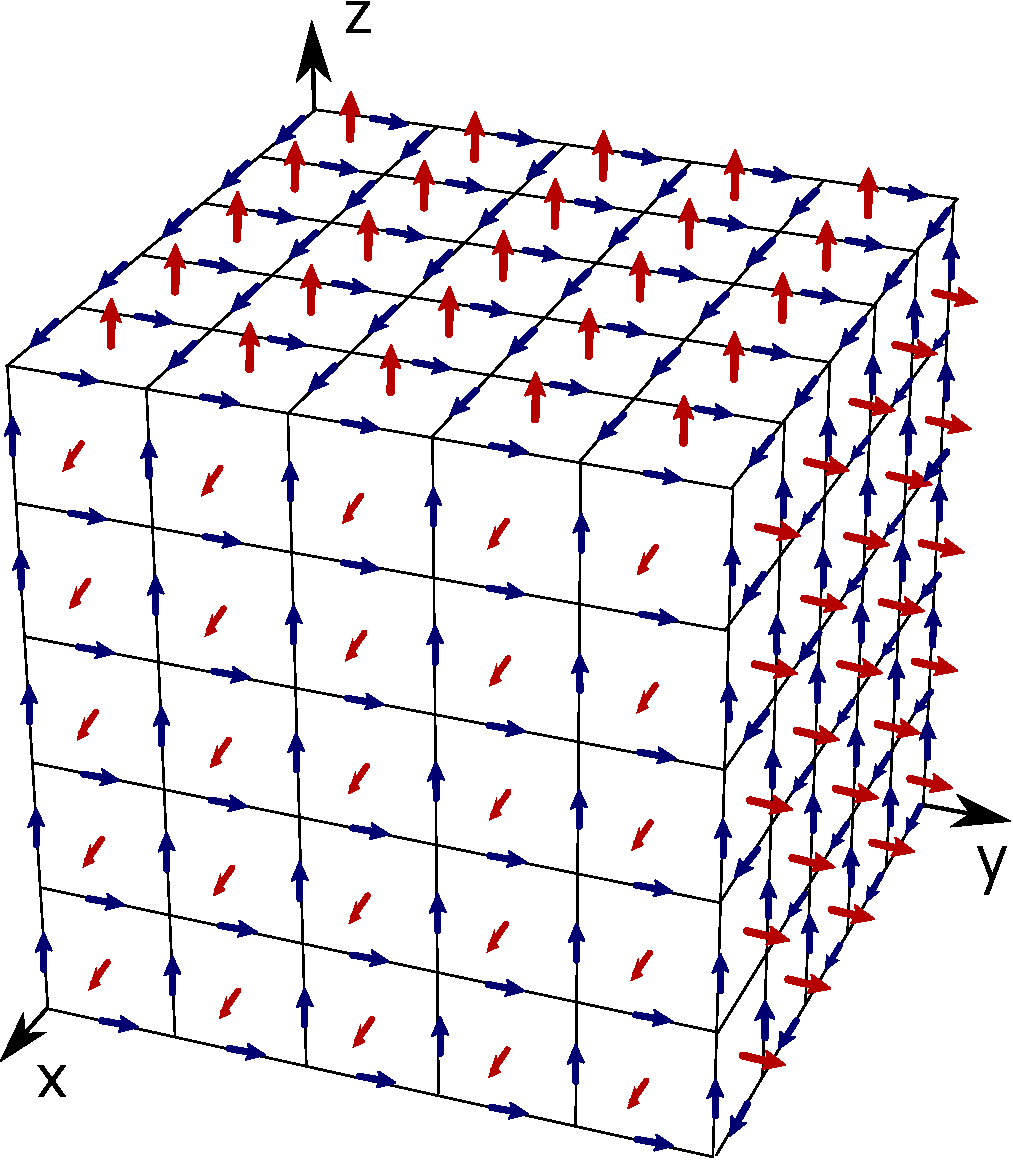
\includegraphics[scale=0.3]{img/analysis/fdtd_mesh}
        \caption{A Yee FDTD grid}
        \label{fig:fdtd-grid}
    \end{subfigure}
    ~
    \begin{subfigure}[b]{0.49\textwidth}
      \centering
        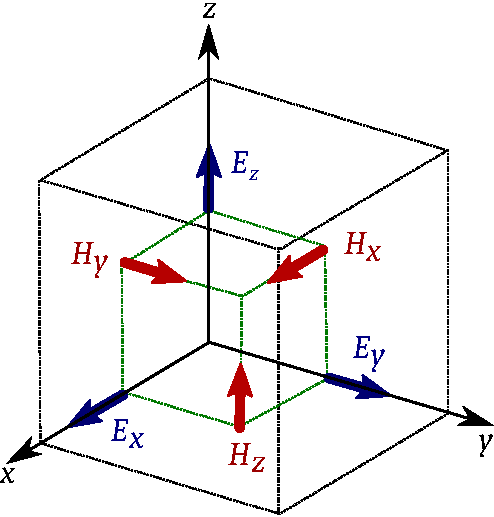
\includegraphics[scale=0.7]{img/analysis/yee_3d}
        \caption{A single Yee cell}
        \label{fig:yee-cell}
    \end{subfigure}
    \caption{Spatial interpetation of the Yee Algorithm}
    \label{fig:space-yee-algorithm}
\end{figure}

The centering of the E- and H-fields in time is often termed the leapfrog method. This time stepping is fully explicit, and thus avoids problems with simultaneous equation and matrix inversions. This leapfrog method is shown in Figure~\ref{fig:leap_frog}. 

\begin{figure}[htbp]
    \centering
    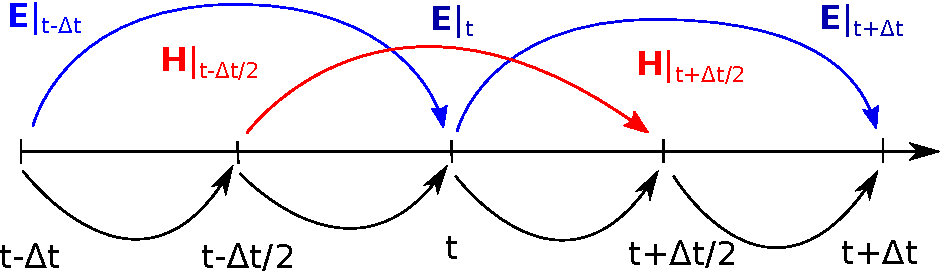
\includegraphics[scale=0.7]{img/analysis/leap_frog}
    \caption{Leap-frog method illustrated on the time line}
    \label{fig:leap_frog}
\end{figure}

To keep an overview, Yee created the following notation which is useful when considering 3D FDTD equations
\begin{align}
  u_X (i \Delta x , j \Delta y, k \Delta z, n \Delta t) = u^n_{X_{i,j,k}}
\end{align}

%http://www.ualr.edu/wirelesslab/fdtd/fdtd3.pdf
\subsubsection{Finite Difference of Maxwell's Equations in 3D}
For completeness the previous ideas and notation can now be used to derive a numerical approximation of Maxwell's Curl Equations in 3D. The derivations will not be shown here, and only the solution for a single Cartesian component will be given here, due to its complexity. As an example, the approximation for $E_x$ is shown below \cite{taflove2000computional},
\begin{align}
  E_x |^{n+1/2}_{i,j+1/2,k+1/2} =& \left( \frac{1-\frac{\sigma_{i,j+1/2,k+1/2} \Delta t}{2\epsilon_{i,j+1/2,k+1/2}}}{1+\frac{\sigma_{i,j+1/2,k+1/2} \Delta t}{2\epsilon_{i,j+1/2,k+1/2}}} \right) E_x |^{n-1/2}_{i,j+1/2,k+1/2}  + \\ 
  &\left(  \frac{\frac{\Delta t}{\epsilon_{i,j+1/2,k+1/2}}}{1+\frac{\sigma_{i,j+1/2,k+1/2} \Delta t}{2\epsilon_{i,j+1/2,k+1/2}} }    \right) \left( \frac{H_z |^n_{i,j+1,k+1/2} - H_z |^n_{i,j,k+1/2} }{\Delta y} - \frac{H_y |^n_{i,j+1/2,k+1} - H_y |^n_{i,j+1/2,k} }{\Delta z} -J_{source}|^n_{i,j+1/2,k+1/2}  \right)
\end{align}

As seen, the equations quickly become large and hard to handle. However, to fully extend this to 3D, this would have to be done for all the the Cartesian coordinates for both E- and H-fields. 

\subsection{Absorbing Boundary Conditions}
Many geometries of interest are defined in open regions, e.g.\ antennas, where the spatial domain is unbounded. Since computers have limited storage, it is needed to find a suitable boundary condition on the outer perimeter of the domain $\Omega$ in order to simulate to infinity. Thus, it is needed to find a boundary condition that allows outward propagating numerical wave to exit the outer perimeter of $\Omega$ without spurious reflections from the outgoing waves. 

One way of achieving the absorbing boundary condition is by terminating the outer boundary with an absorbing material, which is analogous to the method used in anechoic chambers. For this, a perfectly matched layer (PML) is used, which is derived by Berenger \cite{taflove2000computional}. This allows plane waves of arbitrary incidence, polarization, and frequency to be matched at the boundary. PML usually gives a back-reflection in the order of $\approx 10^{-6}$--$10^{-8}$ \cite{taflove2000computional}.

\subsection{FDTD Parameters and Relation to CST}
CST Microwave Studio is used for all simulations in this report. The following will try to connect the FDTD theory to the parameters in CST. Even though CST uses Finite Integration Technique (FIT) instead of finite differences \cite{hirtenfelder2007}. FIT share the structure of FDTD, but uses the Maxwell's Equations on integral form. The advantage of FIT is that it uses less memory and it allows for easier code implementation of some features. Besides this, most of the basic parameters are the same. 

\subsubsection{Cell Size and Meshing}
The choice of cell size is very important when doing FDTD simulations. A general rule of thumb is that a cell should be much less than the smallest wavelength. As a rule of thumb, 10 cells per wavelength is sufficient, that is the cell size should be $\lambda/10$. In advanced FDTD simulations, an adaptive meshing is often used where even smaller cells are used in dense materials with strong-field locations, and large cells outside these areas. When doing this, it is also very important not to change the cell size too much compared to the neighbor cells. It is also necessary that the cell size are small enough to approximate the geometry, which is to be modeled accurately. Geometries such as circles are being approximated with rectangular cells, this causes a ``staircase effect'' on the object, and the representation can be inaccurate if the cell sizes used are too large. 

Another rule of thumb, which can help assessing the right cell size, is that the smallest mechanical item of the structure is to be approximated by at least two cells. The rule of thumb says that \cite{kunz1993fdtd}:
\begin{align}
    \Delta = \frac{d_{\text{min}}}{N_d} 
\end{align}
where 
\begin{where}
\item[$\Delta$] Is the length/width/height of the cell.
\item[$d_{\text{min}}$] Smallest physical dimension.
\item[$N_d$] Oversampling factor -- should be $\geq 1$.
\end{where}

\subsubsection{Time Step Size}
The time step size is another parameter that has to be chosen with care when doing FDTD simulations. The time step should be small enough, such that at any point, a wave should not pass through more than one cell. Calculating the time step is dependent on the cell size, dimensions, and the propagation speed. The time step for the 3D rectangular grid can be calculated as \cite{kunz1993fdtd}:
\begin{align}
   \label{eq:deltat}
   \Delta t &= \frac{1}{c \sqrt{\frac{1}{(\Delta x)^2}+\frac{1}{(\Delta y)^2}+\frac{1}{(\Delta z)^2}}} \\
            &= \frac{1}{c \sqrt{\frac{3}{\Delta^2}}} \\
            &= \frac{\Delta}{c \sqrt{3}}            
\end{align}
where:
\begin{where}
\item [$c$] Speed of light.
\item [$\Delta = \Delta x = \Delta y = \Delta z$] Size of the cell side for rectangular cell.
\end{where}

\subsubsection{Accuracy and Time Limit}
These terms are taken directly from CST Microwave Studio, and are values that limit the simulation either when a certain accuracy criteria has been met or when it has been simulated for a certain amount of time. In practice, it is undesirable that a simulation is stopped due to a given time limit. Therefore, this limit is often set to a very large number. In CST, accuracy is a measure that describes how much energy is left in the system. The accuracy setting makes the simulation stop when a certain energy level, within the structure, has decreased to a chosen level. 

\begin{aautail}
\fixme{tail}
\end{aautail}
